\section{Introduction}
JavaScript is one of the widely used programming languages not only for client-side
but also for server-side programming~\cite{nodejs, meanjs}
and even for small embedded systems~\cite{espruino, tessel2}.
It is the top-ranked language used in active GitHub
repositories\footnote{https://githut.info/}, and \#7 in the TIOBE
Programming Community index\footnote{https://www.tiobe.com/tiobe-index/}.
According to W3Techs\footnote{https://w3techs.com/technologies/details/cp-javascript/all/all},
95.2\% of websites use JavaScript as their client-side programming language.

Despite its popularity, JavaScript developers often suffer from its intricate semantics,
which may cause security vulnerabilities.  For example, calling the following JavaScript
function seems to always return \( \code{false} \):
\begin{lstlisting}[style=myJSstyle]
    function f(x) { return x == !x; }
\end{lstlisting}
Unfortunately, it returns \( \code{true} \) when its argument is an empty array
\( \code{[]} \).  To correctly understand and reason about such complex
behaviors, the formal semantics of JavaScript is necessary.

\begin{figure}
  \centering
  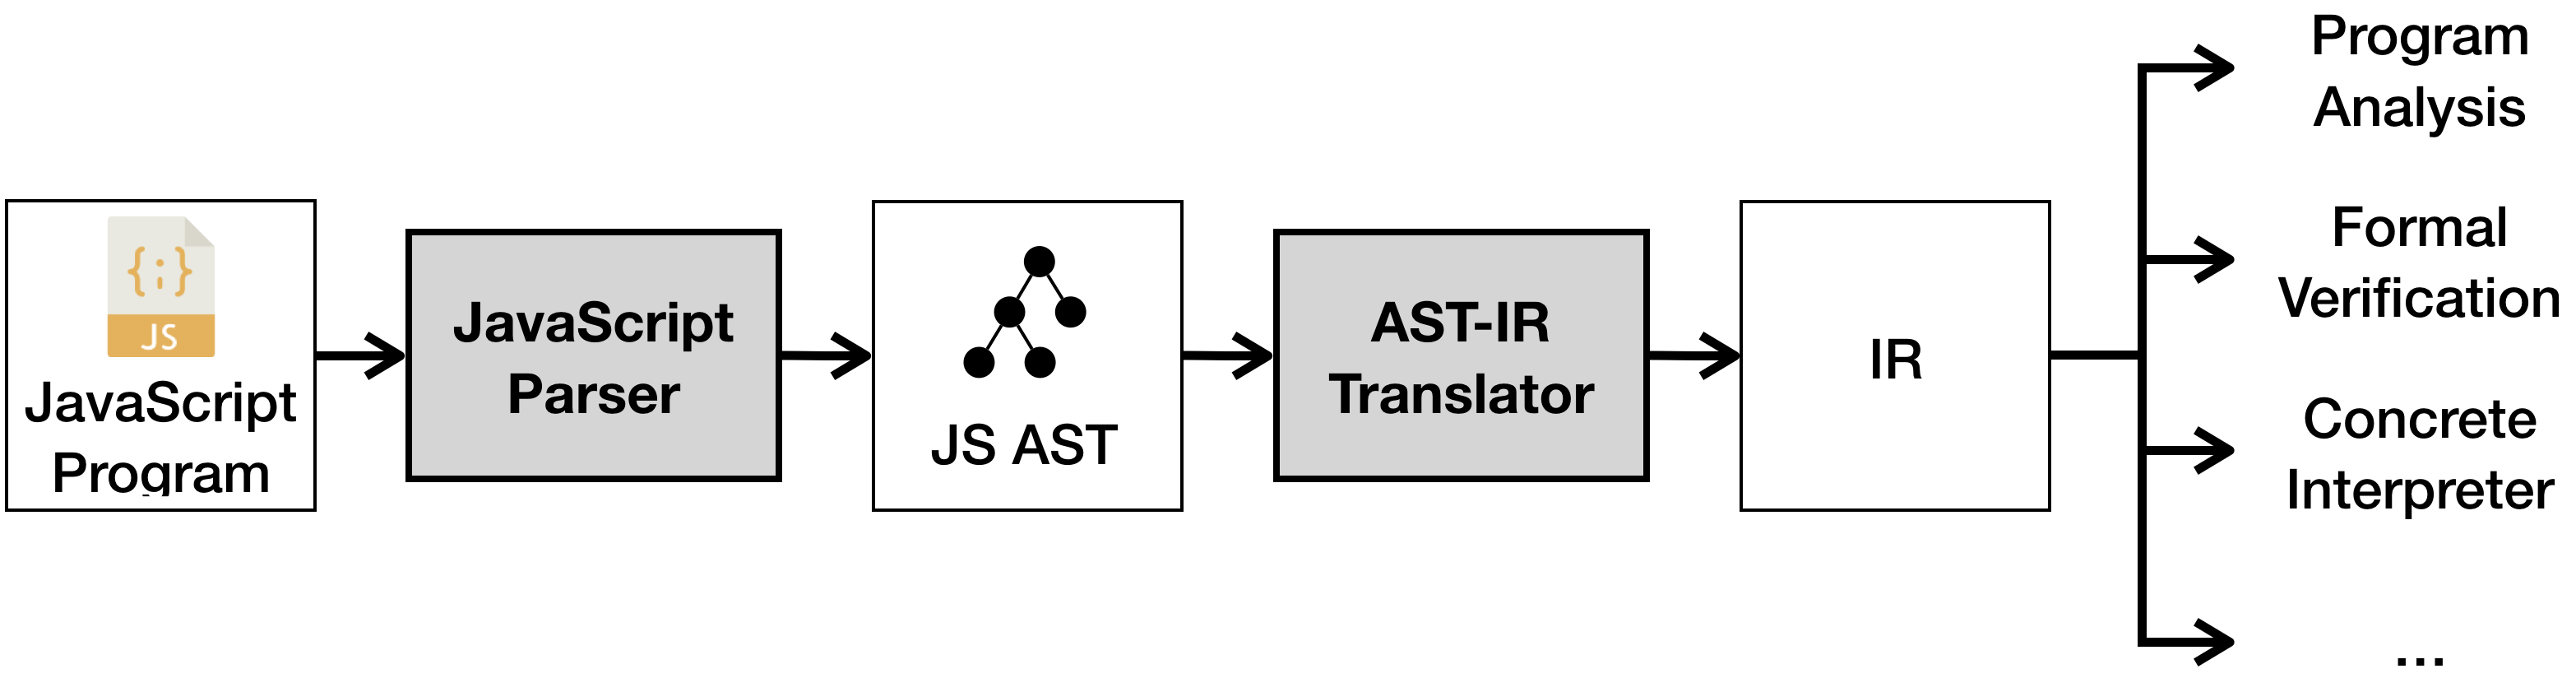
\includegraphics[width=0.48\textwidth]{img/existing.png}
\vspace*{-2em}
  \caption{Existing approaches: Manual extraction of IR-based semantics for ECMAScript}
  \label{fig:existing}
\vspace*{-1em}
\end{figure}

Researchers have defined various JavaScript formal
semantics~\cite{aplas08,lambdajs,kjs,javert} and developed several static
analyzers on top of them~\cite{jsai,tajs,wala,safe}.  As illustrated
in Figure~\ref{fig:existing}, they defined their own Intermediate
Representations (IRs) to represent JavaScript program semantics.  They
built parsers to construct Abstract Syntax Trees (ASTs) from
programs and AST-IR translators to convert ASTs
to their own IRs.  This approach helps researchers focus on IRs
without worrying about diverse and enormous features of JavaScript in
developing new techniques for program analysis and formal verification.
We dub such a methodology that manipulates language semantics by
translating given programs to IRs that are suitable for analysis and
verification \textit{IR-based semantics extraction}.

However, existing approaches to JavaScript IR-based semantics
extraction have difficulties in manipulating recent JavaScript
programs, because they all extract the semantics \textit{manually}.
The JavaScript syntax and semantics are described in the ECMAScript
specification, written in English in a clearly structured and
organized manner.  Unfortunately, manually implementing parsers and
translators for JavaScript from the specification is tedious,
labor-intensive, and error-prone especially because the language is
huge.  The most recent specification, ECMAScript 2019, has 798 pages.

Moreover, manual extraction does not scale for frequent updates of the
specification.  While most existing formal semantics and analyzers of
JavaScript support only ECMAScript 5.1 released in December 2009,
from ECMAScript 6, officially dubbed ECMAScript 2015, the 
ECMAScript specification is updated every year.  Focusing on
ECMAScript 5.1 was reasonable until 2014, because the
specification was rarely updated.  However, in late 2014, The Ecma
Technical Committee 39 (TC39)~\cite{tc39} decided to release the
specification annually.  Currently, no formal semantics
nor analyzers for JavaScript correctly deal with recent ECMAScript
features such as lexical binding via \( \code{let} \), the spread
\( \code{...} \) operator, classes, the \( \code{for-of} \) operator,
the \( \code{async} \) functions, and generators.

In this paper, we propose JavaScript IR-based Semantics Extraction
Toolchain (\( \tool \)), which \textit{automatically} extracts JavaScript
syntax and semantics from the ECMAScript specification.  It
automatically generates a JavaScript parser from the syntax defined in
the ECMAScript specification.  It also automatically extracts the
formal semantics of JavaScript with given \textit{compile rules}.
Each compile rule describes how abstract algorithms in the
specification written in a natural language are converted into
functions of our intermediate representation \( \ires \).  In
addition, to save the labor of defining such compile rules, we also
present a \textit{rule generation assistant}, which suggests new
compile rules based on fault localization of not yet convertible
algorithms.  The assistant helps us deal with changed or newly
introduced algorithms defined in new versions of the ECMAScript
specification as well.

The main contribution of this paper is \( \tool \):
\begin{itemize}[leftmargin=0.5cm]
\item We successfully applied \( \tool \) to ECMAScript 2020, the next
ECMAScript version scheduled to be released in June 2020.  The
automatically extracted semantics passed the official conformance test
suite, Test262~\cite{test262}; out of \inred{XXXXX} tests for
ECMAScript 2020 it passed \inred{XXXXX} tests.
\item \( \tool \) is also applicable to new language features proposed
for a future release to aid language development in a modular way.
Because ECMAScript is an open standard language, various proposals are
available with their own specification changes and tests.  As a case
study, we applied \( \tool \) to such a proposal, during which the tool
found some errors in the proposal.  The reported errors were all confirmed
and the tool passed all the tests.
\item Moreover, since the extraction mechanism of \( \tool \) is fully
automatic, we can use it to find possible specification errors.  We
indeed found 3 specification errors in ECMAScript 2020.  They were all
confirmed by TC39 and will be fixed in the next release.
\end{itemize}
